\documentclass{article}

\usepackage[utf8]{inputenc}

\usepackage{hyperref}

\usepackage{amsmath}
\usepackage{bm}

\usepackage{scrextend}

\usepackage{geometry}
\geometry{
	a4paper,
	total={170mm,257mm},
	left=20mm,
	top=20mm,
}

\usepackage{graphicx}
\usepackage[portuguese]{babel}
\usepackage{subfig}


\usepackage{listings}
\usepackage{xcolor}

\definecolor{codegreen}{rgb}{0,0.6,0}
\definecolor{codegray}{rgb}{0.5,0.5,0.5}
\definecolor{codepurple}{rgb}{0.58,0,0.82}
\definecolor{backcolour}{rgb}{0.95,0.95,0.92}

\lstdefinestyle{mystyle}{
	backgroundcolor=\color{backcolour},   
	commentstyle=\color{codegreen},
	keywordstyle=\color{magenta},
	numberstyle=\tiny\color{codegray},
	stringstyle=\color{codepurple},
	basicstyle=\ttfamily\footnotesize,
	breakatwhitespace=false,         
	breaklines=true,                 
	captionpos=b,                    
	keepspaces=true,                 
	numbers=left,                    
	numbersep=5pt,                  
	showspaces=false,                
	showstringspaces=false,
	showtabs=false,                  
	tabsize=2
}

\lstset{style=mystyle}

%\usepackage{indentfirst}
\setlength{\parindent}{1.5cm}% too much in my eyes delete this
% line and use the default ...


\title{
	Aplicando projeções perspectiva e geométrica (trabalho 4) \\
	\Large Introdução ao Processamento de Imagem Digital \\
	Randerson A. Lemos (103897)
	2022-1S
}

\date{\vspace{-5ex}}

\begin{document}
  \pagenumbering{gobble}
  \maketitle

%
%%
\section{Introdução}
Encontrar a correspondência entre pixels de diferentes imagens que capturam a mesma informação de ângulos, posições e perspectivas diferentes é uma problema muito comum abordado pelo processamento de imagens. Esses problemas são genericamente denominados de problemas de Registro e sua resolução normalmente se desenvolve pelo uso dos conhecimento de álgebra linear e suas ideias de espaços vetoriais e transformações entre tais espaços por meio de matrizes de transformação. Para exemplificar em termos práticos os problemas de registro, observe a Figura \ref{fig:trans} a seguir retirada do material de aula.

\begin{figure}[!htp]%
	\centering
	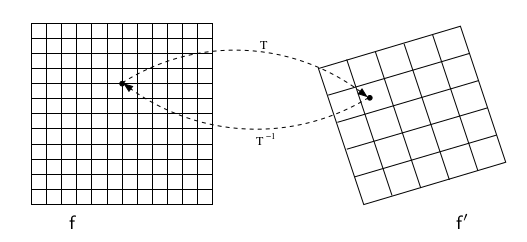
\includegraphics[width=10cm]{transformacao.png}
	\caption{Aplicação da matriz de transformação $\mathbf{T}$ entre as imagens $\mathbf{f}$ e $\mathbf{f'}$ (\textbf{fonte}: material de aula).}%	
	\label{fig:trans}%
\end{figure}

\noindent
Nesse figura, temos duas imagens $\mathbf{f}$ e $\mathbf{f'}$ cujos pixels estão relacionados pela matriz de transformação $\mathbf{T}$, ou seja

\begin{equation}
\mathbf{f'} = \mathbf{T}\mathbf{f}.
\label{eq:trans}
\end{equation}

\noindent
Na Equação \ref{eq:trans}, a matriz de transformação $\mathbf{T}$ está fazendo o mapeamento da imagem $\mathbf{f}$ para a imagem $\mathbf{f'}$. Tal mapeamento pode ser representado como $\mathbf{T}: \mathbf{f} \mapsto \mathbf{f'}$. Um aspecto importante que precisa ser levado em conta nos problemas de registro é o da natureza discreta das informações presentes, isto é: das imagens digitais. Devido a essa natureza, o mapeamento direto $\mathbf{T}: \mathbf{f} \mapsto \mathbf{f'}$ nem sempre vai conduzir um pixel válido da imagem de origem $\mathbf{f}$ para um pixel válido da imagem de destino $\mathbf{f'}$, uma vez que depois de aplicada a matriz de transformação não há garantias que o pixel transformado seja discreto e esteja contido dento do domínio da imagem de destino $\mathbf{f'}$. Para contornar esse aspecto prático da aplicação das matrizes de transformação em domínios discretos, a solução encontrada foi fazer uso da transformação inversa e de métodos de interpolação, isto é:

\begin{equation}
\mathbf{f} = \mathbf{T^{-1}}\mathbf{f'}.
\label{eq:transinv}
\end{equation}

\noindent
A aplicação da transformação inversa garante que todos os pixels da imagem de destino $\mathbf{f'}$ sejam considerados no problema de encontrar seu correspondente na imagem de origem $\mathbf{f}$ e a aplicação das técnicas de interpolação garante que todos os pixels transformados estejam associados a algum pixel válido da imagem de origem $\mathbf{f}$. Existem diversas técnicas de interpolação, sendo algumas das mais conhecidas as seguintes: Interpolação pelo Vizinho Mais Próximo, Interpolação Bilinear, Interpolação Bicúbica e Interpolação por Polinômios de Lagrange. Essas interpolações são amplamente discutidas no material da disciplina como também no documento de instruções desse trabalho.

Os problemas de registro são principalmente organizados em problemas de transformações geométricas e problemas de transformações projetivas. Ambos esses problemas serão discutidos em mais detalhes a seguir.

\subsection{Transformações geométricas}
Os problemas de transformação geométricas consistem de uma transformação espacial e uma interpolação. A transformação espacial está associada as transformações afins de rotação, escala, translações, espelhamento e cisalhamento. Nessas transformações, o paralelismo das linhas e curvas da imagem transformada é preservado, mas dimensões lineares, de área ou volumétricas não. Em coordenadas homogêneas e considerando o caso bidimensional, essas transformações podem ser generalizadas por

\begin{equation}
\begin{bmatrix} 
X'\\
Y'\\
W \\
\end{bmatrix}
=
\begin{bmatrix} 
a & b & c \\
d & e & f \\
g & h & i \\
\end{bmatrix}
%
\begin{bmatrix} 
X \\
Y \\
W \\
\end{bmatrix}.
\label{eq:transexp}
\end{equation}

\noindent
Cada uma das transformações de rotação, escala, translação, espelhamento e cisalhamento terão uma matriz de transformação específica (a matriz com os coeficientes $a,b,\cdots, i$). A seguir, vamos conhecer a forma das matrizes das transformações de escala, translação e rotação.

\subsubsection{Transformação de Escala}
A transformação de escala para o caso 2D pode ser realizada a partir da matriz de transformação em coordenadas homogêneas apresenta a seguir.

\begin{equation}
\begin{bmatrix} 
X'\\
Y'\\
W \\
\end{bmatrix}
=
\begin{bmatrix} 
S_x & 0   & 0 \\
0   & S_y & 0 \\
0   & 0   & 1 \\
\end{bmatrix}
%
\begin{bmatrix} 
X \\
Y \\
W \\
\end{bmatrix}.
\label{eq:transesc}
\end{equation}

\noindent
Então, para aplicar um aumento ou redução de escala da imagem, o usuário precisa definir o valor de escala $S_x$ a ser aplicado ao longo do eixo-x e o valor de escala $S_y$ a ser aplicado ao longo do eixo-y.
 
\subsubsection{Transformação de Translação} 
A transformação de translação para o caso 2D pode ser realizada a partir da matriz de transformação em coordenadas homogêneas apresenta a seguir.

\begin{equation}
\begin{bmatrix} 
X'\\
Y'\\
W \\
\end{bmatrix}
=
\begin{bmatrix} 
1 & 0 & t_x \\
0 & 1 & t_y \\
0 & 0 & 1 \\
\end{bmatrix}
%
\begin{bmatrix} 
X \\
Y \\
W \\
\end{bmatrix}.
\label{eq:transtra}
\end{equation}

\noindent
Então, para aplicar uma translação na imagem, o usuário precisa definir o valor de translação $t_x$ a ser aplicado ao longo do eixo-x e o valor de translação $t_y$ a ser aplicado ao longo do eixo-y.

\subsubsection{Transformação de Rotação} 
A transformação de rotação para o caso 2D pode ser realizada a partir da matriz de transformação em coordenadas homogêneas apresenta a seguir.

\begin{equation}
\begin{bmatrix} 
X'\\
Y'\\
W \\
\end{bmatrix}
=
\begin{bmatrix} 
cos(\alpha) & -sin(\alpha) & 0 \\
sin(\alpha) & cos(\alpha)  & 0 \\
0           & 0            & 1 \\
\end{bmatrix}
%
\begin{bmatrix} 
X \\
Y \\
W \\
\end{bmatrix}.
\label{eq:transrot}
\end{equation}

\noindent
Então, para aplicar uma rotação na imagem, o usuário precisa definir o valor de rotação $\alpha$ a ser aplicado na imagem.

\subsection{Transformações projetivas}
As transformações projetivas estão associadas ao processo de projeção de pontos dispostos tridimensionalmente no espaço em um plano bidimensional. Essas transformações são principalmente do tipo ortográfica ou perspectiva. A projeção ortográfica é uma transformação que realiza o mapeamento de pontos tridimensionais sobre o plano da imagem, tal que os pontos são projetados ao longo de linhas paralelas na imagem (informação extraída do material de aula). Já as projeções perspectivas, apesar de haver o mesmo mapeamento de um espaço tridimensional para um espaço bidimensional (um plano), o tamanho do objecto projeto assim como algumas razões de suas medidas lineares e de área são dependentes do aumento da distância do centro de projeção. Essa dependência está associada a percepção de profundida do sistema visual humano. A ideia das transformações projetivas está apresentada na Figura \ref{fig:transpro}.

\begin{figure}[!htp]%
	\centering
	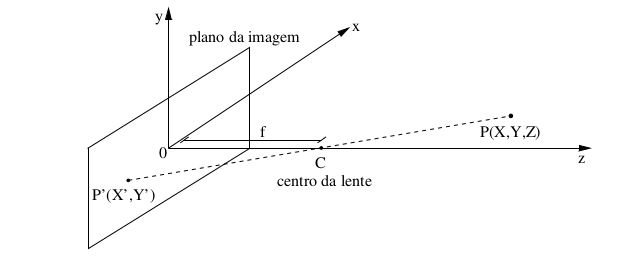
\includegraphics[width=10cm]{transformacaoprojetiva.png}
	\caption{Modelagem geométrica de transformação projetiva (\textbf{fonte}: material de aula).}%	
	\label{fig:transpro}%
\end{figure}

\newpage
Existem algumas maneiras de se calcular a matriz de transformação de uma transformação projetiva. No caso particular das projeções perspectivas, umas das formas de ser obter tal matriz é a partir de quatro pontos não colineares e a resolução das seguintes equações

\begin{equation}
X' = \frac{aX + bY + c}{iX + jY + 1}
\qquad\qquad
Y' = \frac{fX + eY + f}{iX + jY + 1}
\label{eq:transpes}
\end{equation}
considerando-se os quatro pontos não colineares em questão. Os valores obtidos da resolução do sistema de equações para as variáveis $a,b,c,d,e,i,j$ são os coeficientes da matriz de transformação 
\[
\begin{bmatrix} 
	a & b & c \\
	d & e & f \\
	i & j & 1 \\
\end{bmatrix}
\]
da projeção perspectiva em questão.

%
%%
\section{Objetivo}
O objetivo deste documento é o de fornecer uma relatório sobre as técnicas de registro solicitadas no documento de instrução do trabalho 4. De acordo com as instruções, é solicitado que seja desenvolvido um programa capaz de realiza as transformações espaciais de escala e rotação. Também é solicitado a implementação de um programa que realize uma projeção perspectiva sobre a imagem \textbf{baboon\_perspectiva\_result.png}.


%
%%
\section{Solução}
A solução utiliza a linguagem de programação Python e conta com o auxílio do gerenciador de projetos e pacotes Conda. Assumindo que o usuário tenha o Conda instalado em sua máquina, a configuração do projeto pode ser feita pela execução do comando \lstinline{conda env create -f environment.yml} a partir da pasta do projeto \textbf{trab4}. Esse comando cria o ambiente de trabalho \textbf{mc920-trab4} e instala os seguintes módulos: opencv, numpy, scipy, pandas, matplotlib. Finalizada a configuração do ambiente de trabalho em questão, o usuário deve executar o comando \lstinline{source source.sh}\footnote{O comando que configura o ambiente de trabalho mc920-trab4 precisa ser executado apenas um vez. Assim sendo, depois que este ambiente está configurado, o usuário precisa apenas executar o comando \lstinline{source source.sh}} para carregar as variáveis de ambiente adequadas e, assim, poder usar os programas do projeto dentro do próprio ambiente de trabalho recém configurado. 

Dos arquivos presentes na pasta do projeto \textbf{trab4}, destacam-se as pastas \textbf{assets} e \textbf{tex} e os programas \textbf{apply\_perspective.py} e \textbf{main.py}. A pasta \textbf{assets} contém imagens no formato png que podem ser utilizadas para a aplicação das técnicas de registro consideradas. A pasta \textbf{tex} contém os arquivos Latex deste relatório. O programa \textbf{main.py} contém as implementações necessárias para aplicar as técnicas de registro implementadas na imagem de entrada fornecida pelo usuário. Informações pertinentes das implementações serão apresentadas a seguir.

%
\subsection{Apply\_perspective.py}
O programa \textbf{apply\_perspective.py} é responsável pela aplicação da projeção perspectiva requerida no trabalho. Para rodar tal programa, o usuário deve executar o seguinte comando:
\begin{lstlisting}
python3 apply_perspective.py
\end{lstlisting}
\noindent
Depois de executado o programa \textbf{apply\_perspective.py}, a imagem transformada é salva na pasta \textbf{out} com nome adequado e alto explicativo.
\subsubsection{Detalhes de implementação}
A aplicação da transformação perspectiva é realizada com o auxílio da função \textbf{getPerspectiveTransform} disponibilizada pelo módulo do \textbf{opencv}. 
%
\subsection{Main.py}
O programa \textbf{main.py} é responsável pela aplicação de todas as transformações espaciais implementadas. Este programa recebe diferentes parâmetros de entrada e pode ser executado de diferentes maneiras. Para executar transformações de escala com a escolha de uma determina forma de interpolação, o usuário pode usar alguns dos comandos de exemplo a seguir:
\begin{lstlisting}
python3 main.py -imagem_entrada assets/baboon.png -e 1.25 -m lagrange
python3 main.py -imagem_entrada assets/baboon.png -e 1.25 -m bicubic
python3 main.py -imagem_entrada assets/baboon.png -e 1.25 -m bilinear
python3 main.py -imagem_entrada assets/baboon.png -e 1.25 -m nearneighbours
\end{lstlisting}

\noindent
Para executar a transformação de escala por meio da definição dos tamanhos de largura e comprimento, o usuário pode user alguns dos comandos exemplo a seguir:
\begin{lstlisting}
python3 main.py -imagem_entrada assets/baboon.png -d 300x400 -m lagrange
python3 main.py -imagem_entrada assets/baboon.png -d 300x400 -m bicubic
python3 main.py -imagem_entrada assets/baboon.png -d 300x400 -m bilinear
python3 main.py -imagem_entrada assets/baboon.png -d 300x400 -m nearneighbours
\end{lstlisting}

\noindent
Para executar transformações de rotação com a escolha de uma determinada forma de interpolação, o usuário pode usar alguns dos comandos de exemplo a seguir (a unidade considerada para o ângulo de rotação é graus):
\begin{lstlisting}
python3 main.py -imagem_entrada assets/baboon.png -a 1.25 -m lagrange
python3 main.py -imagem_entrada assets/baboon.png -a 1.25 -m bicubic
python3 main.py -imagem_entrada assets/baboon.png -a 1.25 -m bilinear
python3 main.py -imagem_entrada assets/baboon.png -a 1.25 -m nearneighbours
\end{lstlisting}


Em todas as suas diferentes formas de execução, o programa \textbf{main.py} salva na pasta \textbf{out} a imagem transformada com nome adequado e auto explicativo de modo a permitir ao usuátio associar as imagens salvas com as transformações realizadas sobre elas. O programa \textbf{main.py} dispõem das seguintes classes \textbf{Interpolation}, \textbf{Scale} e \textbf{Rotation}. São os grupos de códigos dessas classes que encapsulam as lógicas das interpolações e das transformações de escala e rotação implementadas (logo, não só as implementações das técnicas de interpolação foram feitas, mas também as implementações das técncias de rotação e escala). Maior enfoque será dado a essas classes na sequência.


%
\subsection{Classe Scale}
A classe \textbf{Scale} é responsável pela aplicação da transformação de escala sobre a imagem de entrada. A escala a ser aplicada na imagem de entrada é fornecida pelo usuário e pode ser um fator multiplicativo ou os valores das dimensões finais de largura e altura. Para o primeiro caso o usuário, deve fornecer para o programa principal o parâmetro \textbf{-e} seguido do valor de escala desejado. Para o segundo caso, o usuário deve fornecer o parâmetro de entrada \textbf{-d} seguido das dimensões finais de saída no formado \textbf{Largura x Altura}. Para conseguir aplicar a transformação de escala, essa classe precisa receber uma função capaz de realizar um método de interpolação. Essas funções estão agrupadas na classe \textbf{Interpolation} e serão discutidas mais adiante. A classe \textbf{Scale} retorna a matriz transformada de acordo com o fator de escala fornecido. Essa classe é capaz de realizar transformações de escala considerando valores flutuantes.

%
\subsection{Classe Rotation}
A classe \textbf{Rotation} é resposável pela aplicação da transformação de rotação sobre a imagem de entrada. A rotação a ser aplicada na imagem de entrada é fornecida pelo usuário pelo parâmetro \textbf{-a} seguido do valor de rotação desejado. Para conseguir aplicar a transformação de rotação, essa classe precisa receber uma função capaz de realizar um método de interpolação. A classe \textbf{Rotation} retorna a matriz de transformação de acordo com a fator de rotação fornecido. É imporante salientar que essa classe sempre considera como origem, para aplicação da transformação de rotação, o ponto $(0,0)$ da imagem. Com isso, uma rotação, por exemplo de 30 graus, vai rotacionar a imagem em sentido anti-horário de modo que os pixels que avancem para além do domínio da imagem são descartados. Logo, uma rotação de 45 graus, resulta na perda de 50\% dos valores dos pixels da imagem de entrada e um rotação de 90 graus, resulta na perda de 100\% desses pixels. Essa classe é capaz de realizar transformações de rotação considerando valores flutuantes. Os valores de entrada para essa classe são em graus.

%
\subsection{Classe Interpolation}
A classe \textbf{Interpolation} é responsável por fornecer algumas das funções de interpolação implementadas para as classes \textbf{Scale} e \textbf{Rotation}. Por meio das funções dessas classes, é possível utilizar as seguintes interpolações: Interpolação pelo Vizinho Mais Próximo, Interpolação Bilinear, Interpolação Bicúbica e Interpolação por Polinômios de Lagrange (os detalhes dessas interpolações estão presentes no material da disciplina). Um ponto em comum dessas interpolações é que todas retornam o valor de nível de cinza igual a zero para todos os pixels que caem fora do domínio da imagem de origem.


\section{Resultado}
Os resultados apresentados estão organizados em dois grupos: o primeiro grupo apresenta o resultado gerado pela aplicação da projeção perspectiva requerida no trabalho. O segundo grupo apresenta o resultado gerado pela aplicação de transformações geométricas. 


\subsection{Projeção perspectiva}
A projação perspectiva dos pontos (37, 51), (342, 42), (485, 467), (73, 380) para (0, 0), (511, 0),
(511, 511), (0, 511) aplicada na imagem de entrada da Figura \ref{fig:projpers}

\begin{figure}[!htp]%
	\centering
	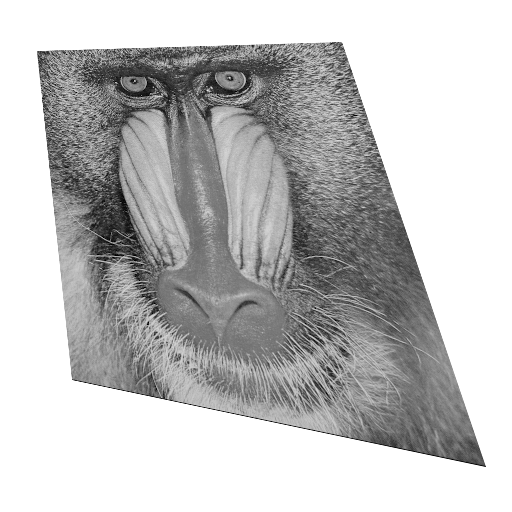
\includegraphics[width=5cm]{baboon_perspectiva.png}
	\caption{Imagem de entrada para aplicação de projeção perspectiva.}%	
	\label{fig:projpers}%
\end{figure}

\noindent
resulta na imagem da Figura \ref{fig:projpersres} a seguir:

\begin{figure}[!htp]%
	\centering
	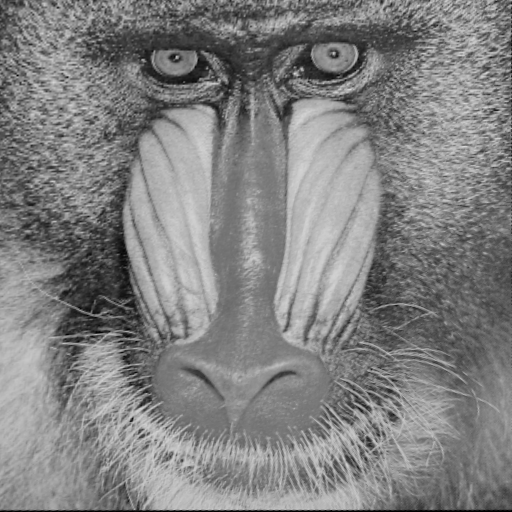
\includegraphics[width=5cm]{baboon_perspectiva_result.png}
	\caption{Imagem resultante da aplicação da projeção perspectiva requerida no trabalho.}%	
	\label{fig:projpersres}%
\end{figure}

\noindent
Podemos ver que a aplicação da projeção perpectiva, resultou no formato original da conhecida imagem \textbf{baboon}.


\subsection{Transformação geométrica}
A seguir apresentaremos o resultado da aplicação das transformações geométricas considerando diferentes técnicas de interpolação. Todas as transformações foram aplicadas sobre a imagem da Figura \ref{fig:projgeoini}.

\begin{figure}[!htp]%
	\centering
	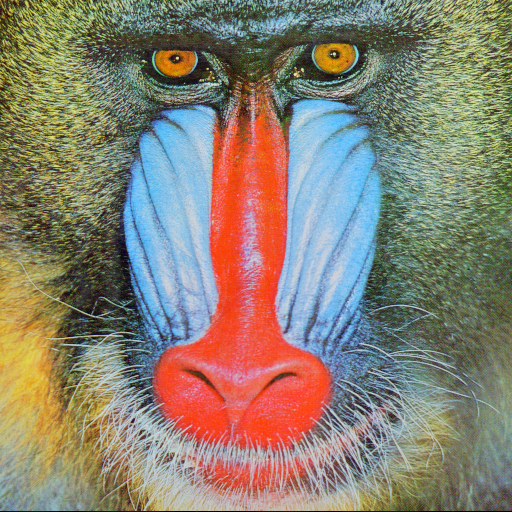
\includegraphics[width=5cm]{baboon.png}
	\caption{Imagem de entrada para aplicação de transformações geométricas.}%	
	\label{fig:projgeoini}%
\end{figure}

\newpage
\subsubsection{Transformação de escala usando o parâmetro -e}
As imagens apresentadas da Figura \ref{fig:escalae} foram obtidas pela aplicação de um fator de escala de $1,25$ considerando as diferentes técnicas de interpolação requeridas.


\begin{figure}[!htp]%
	\centering
	\subfloat[\centering Imagem com nova escala com Interpolação do Vizinho Mais Próximo.]{{ 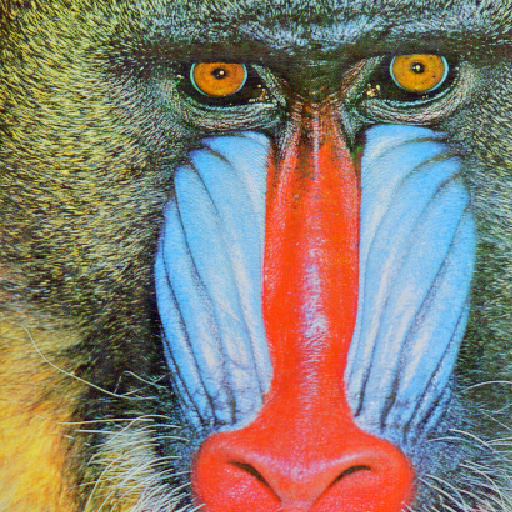
\includegraphics[width=5cm]{baboon_scax_001250_scay_001250_rot_000000_ld_512x512_int_nearneighbours.png} 
	}}%
	%
	\subfloat[\centering Imagem com nova escala com Interpolação Bilinear.]{{ 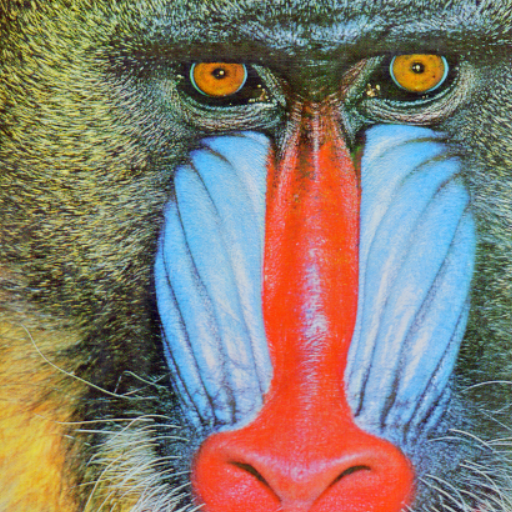
\includegraphics[width=5cm]{baboon_scax_001250_scay_001250_rot_000000_ld_512x512_int_bilinear.png} 
	}}%	
	\\
	\subfloat[\centering Imagem com nova escala com Interpolação Bicubica.]{{ 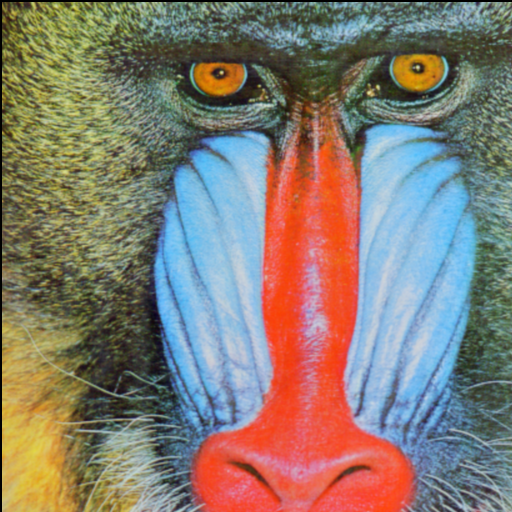
\includegraphics[width=5cm]{baboon_scax_001250_scay_001250_rot_000000_ld_512x512_int_bicubic.png} 
	}}%	
	%
	\subfloat[\centering Imagem com nova escala com Interpolação de Lagrange.]{{ 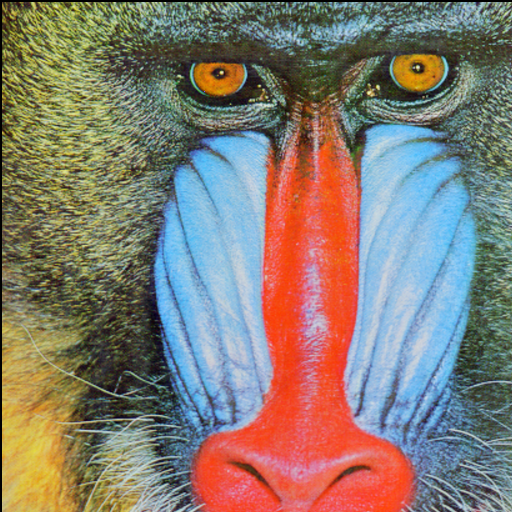
\includegraphics[width=5cm]{baboon_scax_001250_scay_001250_rot_000000_ld_512x512_int_lagrange.png} 
	}}%	
	\caption{Imagens com fator de escala de 1,25 para diferentes métodos de interpolação.}%	
	\label{fig:escalae}%
\end{figure}

\newpage
\subsubsection{Transformação de escala usando o parâmetro -d}
As imagens apresentadas da Figura \ref{fig:escalad} foram obtidas pela aplicação de valores finais de largura 300 e de altura 400 considerando as diferentes tecnicas de interpolação requeridas.


\begin{figure}[!htp]%
	\centering
	\subfloat[\centering Imagem com nova escala com Interpolação do Vizinho Mais Próximo.]{{ 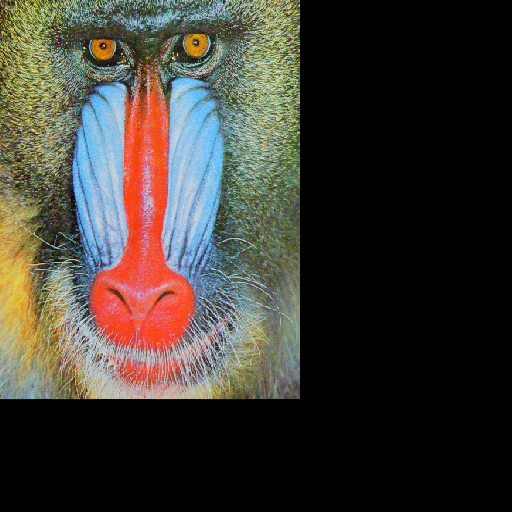
\includegraphics[width=5cm]{baboon_scax_000585_scay_000781_rot_000000_ld_300x400_int_nearneighbours.png} 
	}}%
	%
	\subfloat[\centering Imagem com nova escala com Interpolação Bilinear.]{{ 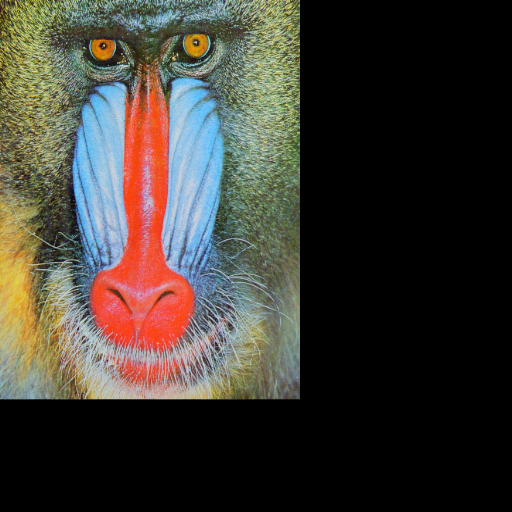
\includegraphics[width=5cm]{baboon_scax_000585_scay_000781_rot_000000_ld_300x400_int_bilinear.png} 
	}}%	
	\\
	\subfloat[\centering Imagem com nova escala com Interpolação Bicubica.]{{ 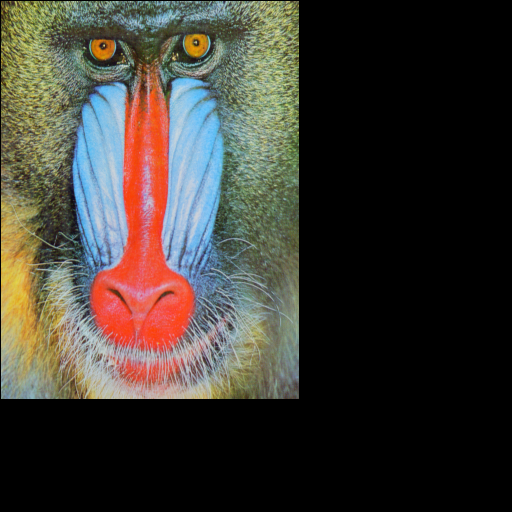
\includegraphics[width=5cm]{baboon_scax_000585_scay_000781_rot_000000_ld_300x400_int_bicubic.png} 
	}}%	
	%
	\subfloat[\centering Imagem com nova escala com Interpolação de Lagrange.]{{ 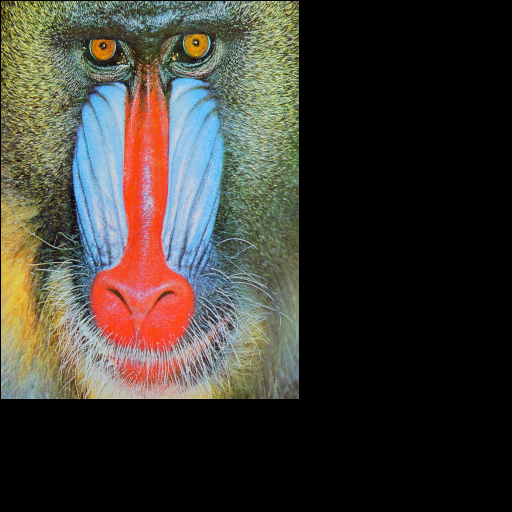
\includegraphics[width=5cm]{baboon_scax_000585_scay_000781_rot_000000_ld_300x400_int_lagrange.png} 
	}}%	
	\caption{Imagens com valores finais de largura 300 e de altura 400 para diferentes métodos de interpolação.}%	
	\label{fig:escalad}%
\end{figure}


\newpage
\subsubsection{Transformação de rotação}
As imagens apresentadas da Figura \ref{fig:rotacao} foram obtidas pela aplicação do valor de rotação de 1,25 graus considerando as diferentes tecnicas de interpolação requeridas.

\begin{figure}[!htp]%
	\centering
	\subfloat[\centering Imagem rotacionada com Interpolação do Vizinho Mais Próximo.]{{ 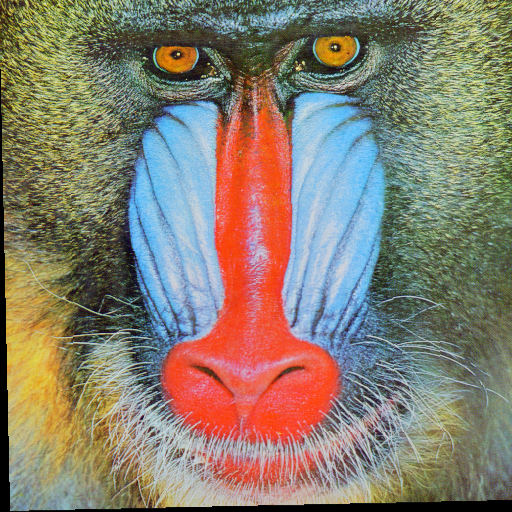
\includegraphics[width=5cm]{baboon_scax_001000_scay_001000_rot_001250_ld_512x512_int_nearneighbours.png} 
	}}%
	%
	\subfloat[\centering Imagem rotacionada com Interpolação Bilinear.]{{ 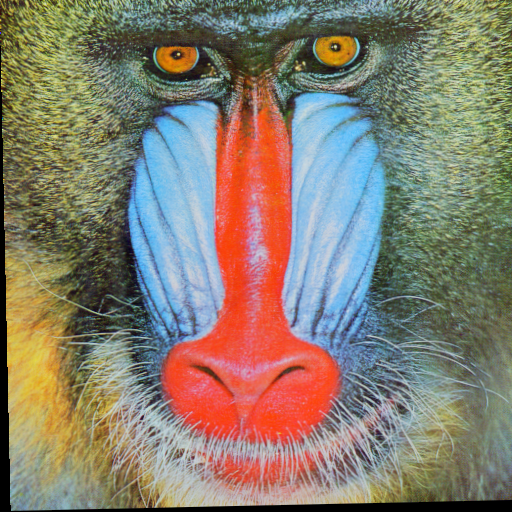
\includegraphics[width=5cm]{baboon_scax_001000_scay_001000_rot_001250_ld_512x512_int_bilinear.png} 
	}}%	
	\\
	\subfloat[\centering Imagem rotacionada com Interpolação Bicubica.]{{ 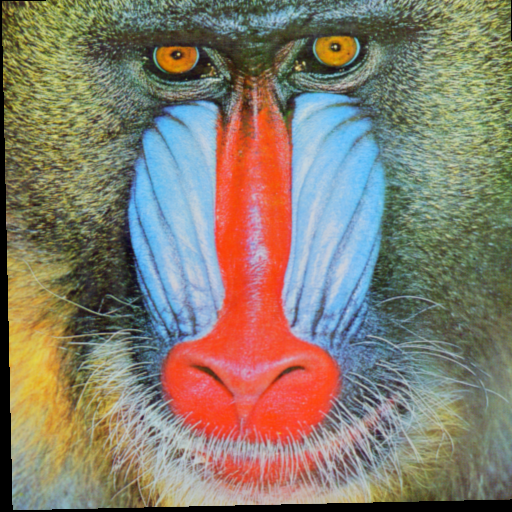
\includegraphics[width=5cm]{baboon_scax_001000_scay_001000_rot_001250_ld_512x512_int_bicubic.png} 
	}}%	
    %
   	\subfloat[\centering Imagem rotacionada com Interpolação de Lagrange.]{{ 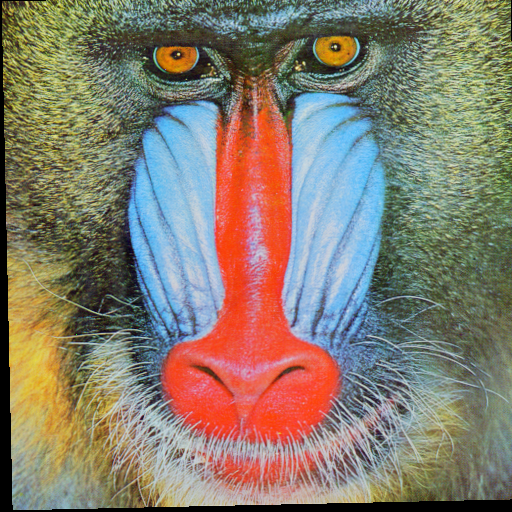
\includegraphics[width=5cm]{baboon_scax_001000_scay_001000_rot_001250_ld_512x512_int_lagrange.png} 
    }}%	
	\caption{Imagens rotacionadas em 1.25 graus para diferentes métodos de interpolação.}%	
	\label{fig:rotacao}%
\end{figure}

%
%%
\section{Discussão e Conclusão}
É possível verificar dos resultados apresentados que as transformações geometricas e projetivas foram implementas e aplicadas corretamente, sendo a mesma afirmação válida para os diferentes tipos de interpolação considerados neste trabalho. Sobre a projeção perspectiva apresentada não resta assunto a ser desenvolvido para além da aplicação correta da técnica dado que a sua implementação foi baseado na utilização de uma função pronta do móludo do \textbf{opencv}. Sobre a transformação geométrica de escala, apesar desta ter sido implementada manualmente, também não resta muito a ser discutido para além da corretudo de sua implementação. Sobre a transformação geométrica de rotação, é válido discutir a forma rudimentar que a aplicação da rotação é feita já que a rotação não é feita com relação ao centro da imagem, mas sim com relação a origem $(0,0)$. Tal forma de realizar a rotação causa um resultado não desejado pelo usuário que provavelmente espera que a rotação da imagem ocorra com relação ao seu ponto central.


Sobre as técnicas de interpolações utilizadas, é pertinente discutir os gastos computacionais e a qualidade das imagens transformadas. Sobre os gastos computacionais, o seu aumento conforme o aumento da sofisticação da técnica de interpolação foi notório. Em ordem crescente de gasto computacional, temos a seguinte disposição das tecnicas de interpolação: Interpolação por Vizinho mais Próximo $<$ Interpolação Bilinear $<$ Interpolação Bicubica $<$ Interpolação de Lagrange. Assim, o uso de técncias mais sofisticadas de interpolação deve ser considerado dentro de projetos específicos e demandas muito particulares uma vez que o uso dessas técnicas impactaram significativamente o desenpenho da solução associada. Sobre a qualidade das imagens resultantes, o autor deste documento particularmente não conseguiu verificar diferenças notáveis. Esse fato corrobora a afirmação de que o uso de técnicas de interpolação mais sofisticadas deve ser considerado dentro de problemas e demandas bem particulares.

\end{document}
